\begin{block}{Results}
\begin{columns}
\begin{column}{.33\textwidth}

    \begin{itemize}
        \item Extraction of major branching ratios from single analysis.
            $\rightarrow$ Full statistical correlation matrix.
        \item Independent of $\sigma_{ZH}$ and $\sigma_{\mathrm{VV-fusion}}$.
        \item Can automatically adapt to BR scenarios
            drastically different from SM.
    \end{itemize}
    \vspace{\baselineskip}
    \begin{table}
        % \resizebox{\textwidth}{!}{
            \InputBiasTable{bias_table.tex}
        % }
        \caption{Fit on the
            expected event counts. In percent. ILD preliminary.}\label{tab:brs}
    \end{table}
\end{column}
\begin{column}{.33\textwidth}
    \begin{figure}
        \centering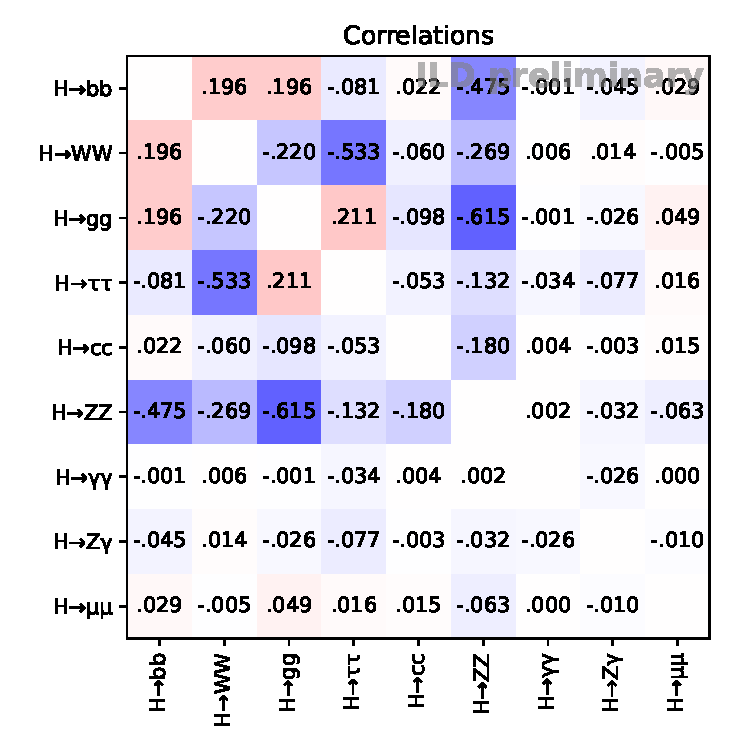
\includegraphics[width=0.7\textwidth]{correlations}
        \caption{Statistical correlations from NLL minimization.}
        \label{fig:correlations}
    \end{figure}
    \begin{figure}
        \centering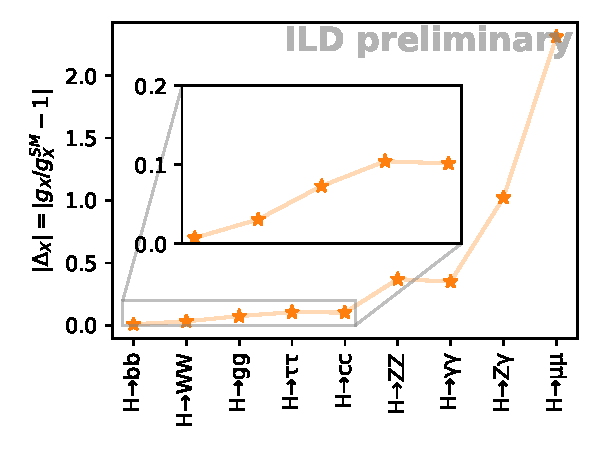
\includegraphics[width=0.7\textwidth]{br_relative_error}
        \caption{Relative BR uncertainty.}
    \end{figure}
\end{column}
\begin{column}{.33\textwidth}
    \begin{figure}
        \centering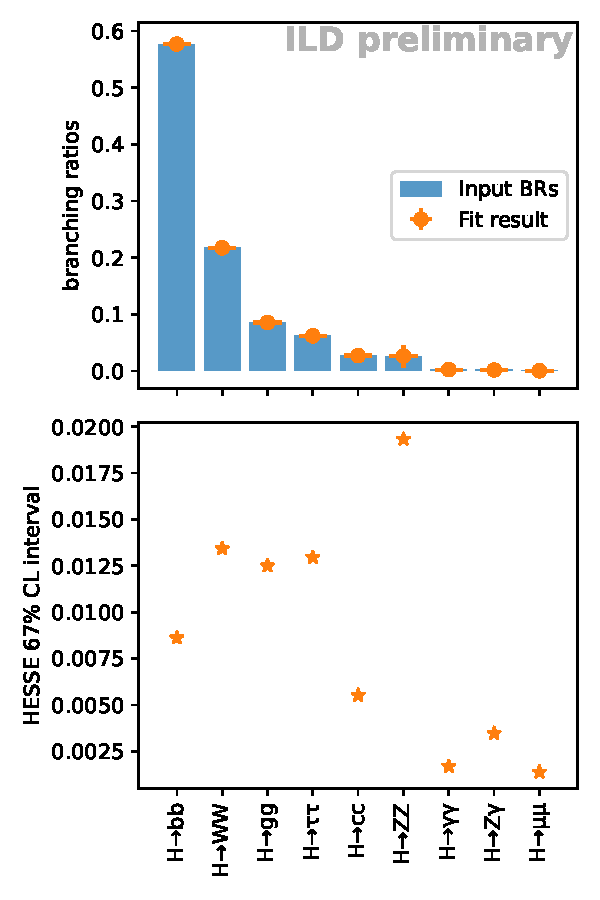
\includegraphics[width=0.7\textwidth]{br_estimates}
        \caption{
            Higgs branching ratios and their uncertainty
            (assuming expected/SM values).
        }
    \end{figure}
\end{column}
\end{columns}
\end{block}
